
\chapter{Fonctionnement}
\label{chap:fonctionnement}

L'algorithme \aes possède deux modes, le premier est le mode courant GCM et le second est le GMAC.

\section{Fonctionnement nominal (GCM)}

\begin{figure}[!h]
  \centering
  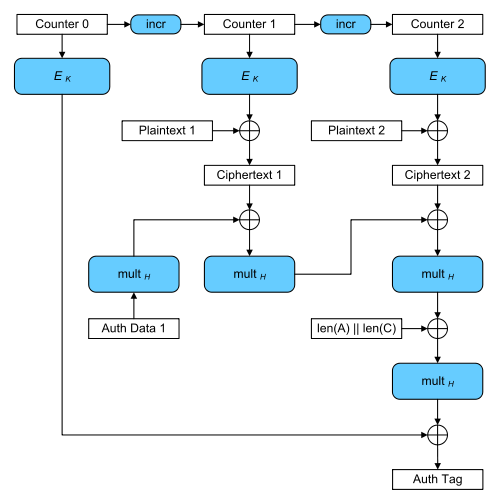
\includegraphics[width=0.8\textwidth]{fonctionnement}
  \caption{Fonctionnement de GCM}
  \label{Fonctionnement de GCM}
\end{figure}

\section{GMAC}



%%% Local Variables: 
%%% mode: latex
%%% TeX-master: "rapport_de_base"
%%% End: 
